\section{Results}
\label{sec:results}

\begin{table*}[t]
\centering\small\setlength{\tabcolsep}{4.5pt}
\fitwidth{\begin{tabular}{lccccccc}
\toprule
System & Accuracy [95\% CI] & Macro-F1 & ECE & \$ / 1k & Lat.\ (s) & $\Delta$ Gem.\ 2.5 ($p$) & $\Delta$ Gem.\ 3.8 ($p$) \\
\midrule
\multicolumn{8}{l}{\emph{Decision models, flat question (one forward pass)}} \\
\quad Liquid d1 Ultra & 67.0 [62.3, 71.4] & 53.5 & 0.044 & 0.18 & 0.46 & +5.7 (0.027) & $-$3.0 (0.22) \\
\quad Perplexity Decider v1.2 & 66.7 [62.1, 71.2] & 56.5 & 0.061 & 0.09 & 0.42 & +5.4 (0.049) & $-$3.2 (0.14) \\
\quad OpenAI GPT-6 Luna Decisions & 66.3 [61.6, 70.9] & 54.7 & 0.059 & 0.41 & 0.35 & +4.9 (0.090) & $-$3.7 (0.13) \\
\quad Baseten Mammoth-1 & 65.8 [61.1, 70.4] & 52.9 & 0.052 & 0$^\P$ & 0.59 & +4.4 (0.10) & $-$4.2 (0.050) \\
\quad Baseten Elephant-1 & 65.3 [60.8, 69.7] & 51.6 & 0.040 & 0$^\P$ & 0.48 & +3.9 (0.16) & $-$4.7 (0.040) \\
\quad Liquid d1 & 62.6 [57.6, 67.2] & 51.5 & 0.075 & 0.08 & 0.41 & +1.2 (0.71) & $-$7.4 (0.002) \\
\quad Jev 1.13 & 61.8 [56.9, 66.5] & 54.9 & 0.103 & 0.19 & 0.26 & +0.5 (0.92) & $-$8.1 ({<}0.001) \\
\quad Perplexity Decider Flash v1.2 & 61.8 [57.1, 66.5] & 49.4 & 0.031 & 0.04 & 0.31 & +0.5 (0.93) & $-$8.1 ({<}0.001) \\
\quad Jev 1.14 & 59.6 [54.7, 64.5] & 53.3 & 0.113 & 0.19 & 0.28 & $-$1.7 (0.56) & $-$10.3 ({<}0.001) \\
\quad Microsoft Decision-1 & 58.1 [53.2, 62.8] & 50.2 & 0.188 & 0.18 & 0.45 & $-$3.2 (0.24) & $-$11.8 ({<}0.001) \\
\quad ScaleDown Classify-1$^\S$ & 50.0 [45.1, 54.9] & 37.4 & 0.090 & 0.24 & 0.72 & $-$11.3 ({<}0.001) & $-$20.0 ({<}0.001) \\
\multicolumn{8}{l}{\emph{Generative LLMs, the paper's prompt}} \\
\quad Gemini 2.5 Flash, thinking off & 61.3 [56.7, 66.0] & 53.1 & -- & 1.66 & 1.55 & -- & $-$8.6 ({<}0.001) \\
\quad Gemini 2.5 Flash, thinking on & 57.9 [53.0, 62.8] & 51.4 & -- & 6.04 & 9.57 & $-$3.4 (0.19) & $-$12.1 ({<}0.001) \\
\quad Gemini 3.8 Flash, thinking low & 70.0 [65.5, 74.4] & 61.3 & -- & 3.65 & 2.18 & +8.6 ({<}0.001) & -- \\
\quad Gemini 3.8 Flash, default thinking & 66.7 [62.1, 71.2] & 59.4 & -- & 5.51 & 5.01 & +5.4 (0.043) & $-$3.2 (0.019) \\
\midrule
\quad Gemini 2.5 Flash, as published$^\ddagger$ & 65.3 & -- & -- & -- & -- & -- & -- \\
\bottomrule
\end{tabular}}
\caption{Conflict-type classification on the \conflicts test split ($n=406$), five classes, sorted by accuracy. Every system sees the same inputs; the LLMs receive the paper's prompt verbatim and the decision models a choice question with the same instructions, definitions and examples. Cost: billed cost per 1,000 queries through one gateway (USD). Latency: mean per query. ECE is undefined for text answers. $\Delta$: accuracy difference in points from Gemini~2.5 Flash (thinking off, the paper's setup) and from Gemini~3.8 Flash (thinking low), exact McNemar $p$. $^\S$Its API accepts only a single text field, so it receives the same content as one text (the LLMs' numbered results). $^\P$Free on the gateway at the time of the runs (billed \$0). $^\ddagger$Reported by \citet{cattan2025dragged} on all 458 queries; not comparable query by query.}
\label{tab:main}
\end{table*}


\subsection{\jev against the LLMs}
\label{sec:main}

Table~\ref{tab:main} gives the main comparison. Asked directly, \jev 1.13 classifies \jevacc\% of test queries
correctly [\jevlo, \jevhi]. Gemini~2.5 Flash with the paper's prompt reaches \gtwofiveacc\% on the same queries;
the difference is \jevvstwofivediff points [\jevvstwofivelo, \jevvstwofivehi] ($p\jevvstwofivep$). \jev does this
at \$\jevcost per thousand queries against \$\gtwofivecost (\costratiotwofive$\times$ cheaper) and in
\jevlat\,s against \gtwofivelat\,s (\latratiotwofive$\times$ faster). It is the fastest of the \nconfigs model
configurations we ran; the fastest non-\jev configuration takes \fastestother\,s.

The current Gemini~3.8 Flash is clearly stronger: at its lowest thinking level it reaches \gthreeeightacc\%, and
\jev's difference from it is \jevvsthreeeightdiff points [\jevvsthreeeightlo, \jevvsthreeeighthi] ($p\jevvsthreeeightp$), at
\costratiothreeeight$\times$ \jev's cost and \latratiothreeeight$\times$ its latency. More thinking does not help
either Gemini: Gemini~3.8 Flash at its default level scores \gthreeeightdefaultacc\% ($p\gthinkvsnothinkp$ against
the low level) and Gemini~2.5 Flash with thinking \gtwofivethinkacc\% ($p\gtwofivethinkvsnothinkp$).

\paragraph{Reproducing the published number.} On all \nall queries, the scope of the published result, our rerun of
Gemini~2.5 Flash scores \allgtwofive\% against the published 65.3\%, and \jev \alljev\%. The hosted model may have
changed since publication, and the paper does not specify how results were joined in the prompt or whether thinking
was enabled. We therefore compare \jev with our rerun on identical inputs and report the published figure only as
context.

\begin{table}[t]
\centering\footnotesize\setlength{\tabcolsep}{3pt}
\fitwidth{\begin{tabular}{lccccc}
\toprule
F1 & NC & Comp.\ & Opin.\ & Outd.\ & Mis. \\
\midrule
Liquid d1 Ultra & 69.2 & 57.3 & 78.2 & 62.7 & 0.0 \\
Perplexity v1.2 & 67.5 & 59.4 & 76.4 & 67.2 & 11.8 \\
GPT-6 Luna & 70.0 & 67.2 & 63.7 & 72.7 & 0.0 \\
Mammoth-1 & 68.9 & 54.5 & 78.5 & 62.5 & 0.0 \\
Elephant-1 & 69.6 & 59.5 & 70.2 & 58.5 & 0.0 \\
Liquid d1 & 63.0 & 58.4 & 69.8 & 66.2 & 0.0 \\
Jev 1.13 & 64.0 & 62.7 & 72.5 & 65.0 & 10.2 \\
Perplexity Flash v1.2 & 66.9 & 53.6 & 69.1 & 57.7 & 0.0 \\
Jev 1.14 & 59.2 & 63.3 & 73.7 & 61.3 & 9.0 \\
Microsoft D-1 & 51.6 & 58.5 & 77.0 & 59.4 & 4.5 \\
ScaleDown C-1$^\S$ & 60.0 & 42.3 & 57.3 & 27.5 & 0.0 \\
\midrule
Gemini 2.5 (off) & 60.9 & 59.7 & 76.2 & 59.0 & 9.8 \\
Gemini 3.8 (low) & 71.8 & 68.3 & 75.1 & 66.1 & 25.0 \\
\bottomrule
\end{tabular}}
\caption{Per-class F1 on the test split (support: No conflict 143, Complementary 102, Opinions 102, Outdated 55, Misinformation 4): decision models with the flat question, then Gemini~2.5 Flash (thinking off) and Gemini~3.8 Flash (thinking low). $^\S$Its API accepts only a single text field, so it receives the same content as one text (the LLMs' numbered results).}
\label{tab:perclass}
\end{table}


\paragraph{Where \jev is strong and weak.} Per class (Table~\ref{tab:perclass}), flat \jev is strongest on
\emph{Outdated information} (F1 \jevoutdf, against \gthreeeightoutdf for Gemini~3.8 Flash) and weakest, like every
system, on \emph{Misinformation}, which has \nmisitest test instances. Its probabilities are informative but
over-confident: the mean top probability is \flatmeanconf\% at \jevacc\% accuracy (ECE \jevece).

\subsection{Flat or tree?}
\label{sec:formulation}

Decomposing the taxonomy into yes/no questions fails. Tree v1 reaches \treeoneacc\%, \flatvstreediffabs points below
the flat question ($p\flatvstreep$), with a macro-F1 of \mftreeone. The failure is concentrated: tree v1 labels
\testopintocomp of the \testnopin \emph{Conflicting opinions} test queries as \emph{Complementary} (F1
\treeoneopinf for opinions). We had seen the cause on the development split: \jev answers the \emph{compatible}
question \emph{yes} for opinion topics almost as readily as for complementary ones (mean probability
\devcompatopin vs.\ \devcompatcomp), sending \devopintocomp of \devnopin development opinion queries the wrong way,
while the \emph{opinion} question separates the two classes well (AUROC \devopinionauroc). The \emph{misinformation}
question shows the yes-bias reported for batched yes/no questions \citep{deusser2026jev}: its mean probability
ranged from \devmisinfolo to \devmisinfohi across all five classes.

Tree v2 asks \emph{opinion} first and treats misinformation as the residual factual conflict. On the test split it
reaches \treetwoacc\%, tied with flat ($p\flatvstreevtwop$), and is much better calibrated (ECE \treetwoece vs.\
\jevece). Its weaknesses are the price of the revision: it rarely predicts \emph{Outdated} (F1 \treetwooutdf) and,
as \S\ref{sec:diagnostics} shows, it misses planted misinformation. It also does not transfer: applied unchanged to
the other decision models it helps Perplexity's model, leaves Microsoft's within noise, and hurts Liquid's and GPT-6-luna's (Table~\ref{tab:decision_models}).
We therefore treat the flat question as \jev's primary format and tree v2 as a \jev-specific variant.

\subsection{A confidence-gated cascade}
\label{sec:cascade}

\begin{table*}[t]
\centering\small
\fitwidth{\begin{tabular}{lcccccc}
\toprule
$f$ & Acc. & Random & $\Delta$ vs LLM [95\% CI] & $p$ & Cost & Lat.\ (s) \\
\midrule
\multicolumn{7}{l}{\emph{Cheap stage: Jev 1.13, flat} (AUROC of confidence 0.70)} \\
\quad 0\% & 61.8 & 61.8 & $-$8.1 [$-$12.3, $-$3.9] & {<}0.001 & 5\% & 0.26 \\
\quad 10\% & 66.3 & 62.6 & $-$3.7 [$-$7.4, +0.0] & 0.07 & 16\% & 0.47 \\
\quad 25\% & 68.5 & 63.9 & $-$1.5 [$-$4.4, +1.5] & 0.41 & 30\% & 0.81 \\
\quad 50\% & 69.2 & 65.9 & $-$0.7 [$-$2.7, +1.0] & 0.61 & 54\% & 1.34 \\
\multicolumn{7}{l}{\emph{Cheap stage: Jev 1.13, tree v2$^\dagger$} (AUROC of confidence 0.73)} \\
\quad 0\% & 63.5 & 63.5 & $-$6.4 [$-$11.6, $-$1.5] & 0.02 & 5\% & 0.25 \\
\quad 10\% & 65.0 & 64.2 & $-$4.9 [$-$9.6, $-$0.2] & 0.05 & 15\% & 0.48 \\
\quad 25\% & 68.5 & 65.2 & $-$1.5 [$-$5.4, +2.5] & 0.54 & 29\% & 0.81 \\
\quad 50\% & 71.4 & 66.7 & +1.5 [$-$0.7, +3.9] & 0.31 & 54\% & 1.33 \\
\multicolumn{7}{l}{\emph{Cheap stage: Jev 1.14, flat} (AUROC of confidence 0.70)} \\
\quad 0\% & 59.6 & 59.6 & $-$10.3 [$-$14.8, $-$5.9] & {<}0.001 & 5\% & 0.28 \\
\quad 10\% & 64.0 & 60.7 & $-$5.9 [$-$9.9, $-$2.0] & 0.004 & 15\% & 0.49 \\
\quad 25\% & 65.8 & 62.2 & $-$4.2 [$-$7.4, $-$1.0] & 0.02 & 30\% & 0.82 \\
\quad 50\% & 68.7 & 64.8 & $-$1.2 [$-$3.4, +1.0] & 0.36 & 54\% & 1.36 \\
\bottomrule
\end{tabular}}
\caption{Confidence-gated cascade: the fraction $f$ of queries with the lowest Jev top probability goes to Gemini 3.8 Flash (thinking low; 70.0\% alone). \emph{Random}: expected accuracy when the same number of queries is escalated at random. Cost is relative to the LLM alone. Thresholds are label-free quantiles, fixed before computing. $^\dagger$Revised on development data.}
\label{tab:cascade}
\end{table*}


\jev's confidence ranks its own errors (AUROC \cascflatauroc for flat, \casctreeauroc for tree v2), which makes it
a natural first stage before an LLM. Table~\ref{tab:cascade} and Figure~\ref{fig:cascade} show the result.
Escalating 10\% of queries to Gemini~3.8 Flash already lifts flat \jev from \cascflatzeroacc\% to
\cascflattenacc\% at \cascflattencost\% of the LLM's cost. At the pre-specified 25\% the cascade reaches
\cascflattfacc\%, a difference of \cascflattfdiff points from the LLM alone [\cascflattflo, \cascflattfhi] ($p\cascflattfp$), at
\cascflattfcost\% of its cost and \cascflattflat\,s mean latency. Escalating by confidence beats escalating at
random at every fraction (\cascflattfacc\% vs.\ \cascflattfrand\% at 25\%). With tree v2 as the first stage, the
cascade at 50\% scores \casctreefiftyacc\%, numerically above the LLM alone ($p\casctreefiftyp$), because \jev is
right on some queries the LLM gets wrong; we read this as a trend, not a gain.

The interval at 25\% rules out a loss larger than \cascflattfloabs points relative to the LLM; showing formal
equivalence at a tighter margin would need more queries than \conflicts provides.

\begin{figure*}[t]
\centering
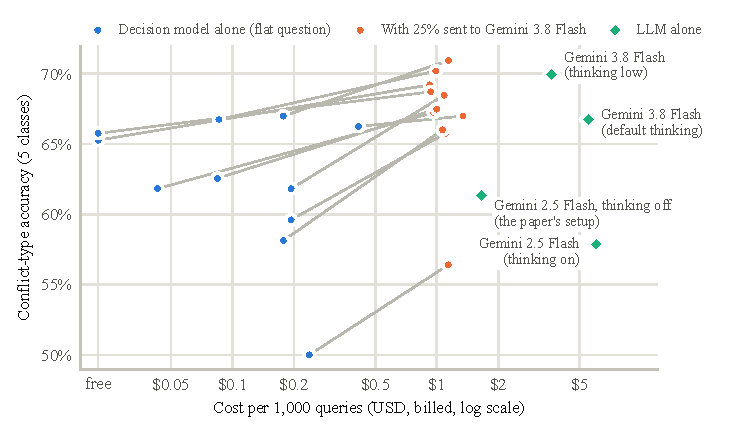
\includegraphics[width=0.78\textwidth]{figures/cascade_cost_accuracy.pdf}
\caption{Accuracy against cost (log scale) on the test split. Curves: \jev answers first and the least confident
fraction of queries goes to Gemini~3.8 Flash; dots mark 25\% and 50\% escalated (at 25\% the two curves nearly
coincide). Diamonds: LLMs alone with the paper's prompt.}
\label{fig:cascade}
\end{figure*}

\subsection{Diagnostics}
\label{sec:diagnostics}

We specified three hypotheses and their tests before running them; Tables~\ref{tab:diagnostics}
and~\ref{tab:plant} give the results. An identical rerun sets the noise floor: no system is deterministic, and
\jev changes its predicted type on \diagjfrerunflip\% of queries with nothing changed (Gemini~3.8 Flash:
\diaggmrerunflip\%).

\begin{table*}[t]
\centering\footnotesize\setlength{\tabcolsep}{4pt}
\fitwidth{\begin{tabular}{lccccccccc}
\toprule
 & \multicolumn{3}{c}{Jev flat} & \multicolumn{3}{c}{Jev tree v2$^\dagger$} & \multicolumn{3}{c}{Gemini 3.8} \\
\cmidrule(lr){2-4}\cmidrule(lr){5-7}\cmidrule(lr){8-10}
Perturbation & $\Delta$Acc ($p$) & Flip & Outd. & $\Delta$Acc ($p$) & Flip & Outd. & $\Delta$Acc ($p$) & Flip & Outd. \\
\midrule
Rerun & $-$0.5 (0.69) & 2.0 & 74.5 & $-$0.2 (1.00) & 2.5 & 20.0 & +1.2 (0.27) & 3.4 & 72.7 \\
No dates & $-$1.0 (0.34) & 3.0 & 74.5 & +0.0 (1.00) & 3.4 & 20.0 & $-$0.7 (0.51) & 2.7 & 67.3 \\
Recency in code & +0.2 (1.00) & 3.4 & 76.4 & +0.2 (1.00) & 3.7 & 21.8 & $-$0.7 (0.65) & 5.7 & 72.7 \\
Shuffle, seed 1 & +1.5 (0.38) & 11.1 & 72.7 & $-$1.5 (0.33) & 9.9 & 18.2 & $-$0.5 (0.85) & 8.4 & 74.5 \\
Shuffle, seed 2 & +0.2 (1.00) & 12.1 & 67.3 & $-$2.2 (0.11) & 8.4 & 18.2 & $-$2.7 (0.09) & 10.3 & 70.9 \\
\midrule
Original Outd.\ recall & \multicolumn{3}{c}{72.7} & \multicolumn{3}{c}{20.0} & \multicolumn{3}{c}{69.1} \\
\bottomrule
\end{tabular}}
\caption{Diagnostics on the test split. Each perturbed run is compared with the same system's original run. $\Delta$Acc: accuracy change in points (exact McNemar $p$). Flip: share of queries whose predicted type changed (\%). Outd.: recall (\%) on the 55 \emph{Outdated} queries after the perturbation. The identical rerun is the noise floor. $^\dagger$Revised on development data.}
\label{tab:diagnostics}
\end{table*}


\paragraph{Dates do not matter.} \jev's documentation lists ordering dates as a known weakness
\citep{typesafe2026jagged}, and we expected it to explain errors on \emph{Outdated}. It does not. Removing every
date changes no system's accuracy beyond the noise floor (\jev: \diagjfnodatesdiff points, $p\diagjfnodatesp$;
Gemini: \diaggmnodatesdiff, $p\diaggmnodatesp$), and neither does adding each result's recency rank computed in
code. \jev's recall on \emph{Outdated} is \diagjforigrec\% originally, \diagjfnodatesrec\% without dates and
\diagjfdatesincoderec\% with code-computed recency, at or above Gemini's in every condition. The systems recognise
outdated sources from their content (phrases such as ``former'' or ``as of'', and conflicting values), not from
publication dates. The weak \emph{Outdated} score of tree v2 comes from its question design, not from dates.

\paragraph{Order sensitivity is real but not specific to \jev.} Shuffling the results changes \jev's predicted type
on \diagjfshuffleflip\% of queries [\diagjfshufflelo, \diagjfshufflehi] over both seeds, well above its
\diagjfrerunflip\% noise floor; Gemini~3.8 Flash flips on \diaggmshuffleflip\%
[\diaggmshufflelo, \diaggmshufflehi]. On the same shuffles the two do not differ ($p\diagflipjevvsgonep$ and $p\diagflipjevvsgtwop$). Accuracy moves by at most a few points in either direction.

\begin{table*}[t]
\centering\small
\fitwidth{\begin{tabular}{lccccc}
\toprule
System & Hit & False al. & Youden & Any conflict & AUROC \\
\midrule
Jev 1.13, flat & 66.7 & 17.7 & +0.490 & 85.4 / 41.7 & 0.81 \\
Jev 1.13, tree v2$^\dagger$ & 19.8 & 2.1 & +0.177 & 67.7 / 25.0 & 0.70 \\
Gemini 3.8 Flash (low) & 52.1 & 3.1 & +0.490 & 71.9 / 25.0 & -- \\
\bottomrule
\end{tabular}}
\caption{One planted false source in 96 \emph{No conflict} test queries (expected label: \emph{Misinformation}). Hit: planted copy labelled Misinformation. False al.: clean copy of the same query labelled Misinformation. Youden = hit $-$ false alarm. Any conflict: planted / clean copy not labelled No conflict. AUROC: P(Misinformation) separating planted from clean copies. $^\dagger$Revised on development data.}
\label{tab:plant}
\end{table*}


\paragraph{A planted false source is noticed as well as by the LLM.} \conflicts has too few \emph{Misinformation}
queries to evaluate. We construct them: in \nplant \emph{No conflict} test queries whose gold answer appears in some
result, we rewrite one such result so that it states a plausible wrong answer, produced by a third model
(GPT-4.1-mini) so that neither classifier judges its own text. The expected label becomes \emph{Misinformation}.
Flat \jev labels \plantjfhit\% of planted queries as misinformation against \plantgmhit\% for Gemini~3.8 Flash
($p\planthitp$), but it also does so for \plantjffa\% of the clean versions of the same queries against
\plantgmfa\% ($p\plantfap$). Net of false alarms the two are identical (Youden \plantjfyouden each; difference
\plantyoudendiff [\plantyoudenlo, \plantyoudenhi]). \jev's misinformation probability separates planted from clean
versions with AUROC \plantjfauroc, so a threshold can trade detections for fewer false alarms. Tree v2, whose
misinformation rule was chosen on a development split with a single misinformation query, detects only
\plantjthit\%.

\subsection{Robustness across versions and decision models}
\label{sec:robustness}

\paragraph{\jev 1.14.} The newer version behaves like 1.13 (Table~\ref{tab:main}): \onefouracc\% with the flat
question (\onefourvsonethreediff points, $p\onefourvsonethreep$) and \onefourtreeacc\% with tree v2
($p\onefourtreevsonethreep$), still tied with Gemini~2.5 Flash ($p\onefourvstwofivep$), with the same failure
of tree v1 and the same cascade behaviour (tree v2 at 50\%: \onefourcascfiftyacc\%, $p\onefourcascfiftyp$ against
the LLM alone).

\begin{table*}[t]
\centering\small\setlength{\tabcolsep}{5pt}
\fitwidth{\begin{tabular}{lccccccc}
\toprule
Decision model & Flat & Tree v2 & ECE & \$ / 1k & Lat.\ (s) & $\Delta$ Jev ($p$) & $\Delta$ Gemini 3.8 ($p$) \\
\midrule
Jev 1.13 & 61.8 & 63.5 & 0.103 & 0.19 & 0.26 & -- & $-$8.1 ({<}0.001) \\
Perplexity v1.2 & 66.7 & 69.0 & 0.061 & 0.09 & 0.42 & +4.9 (0.03) & $-$3.2 (0.14) \\
GPT-6-luna & 66.3 & 50.0 & 0.059 & 0.41 & 0.35 & +4.4 (0.11) & $-$3.7 (0.13) \\
Liquid d1 & 62.6 & 58.4 & 0.075 & 0.08 & 0.41 & +0.7 (0.83) & $-$7.4 (0.002) \\
Microsoft d-1 & 58.1 & 57.4 & 0.188 & 0.18 & 0.45 & $-$3.7 (0.13) & $-$11.8 ({<}0.001) \\
\bottomrule
\end{tabular}}
\caption{Jev against the other decision models available through the same gateway, with Jev's frozen questions and inputs, nothing tuned per model (test split). Flat, Tree v2: accuracy (\%). ECE and latency for the flat question. $\Delta$: accuracy difference of the flat question from Jev and from Gemini~3.8 Flash in points, with exact McNemar $p$. Models: Perplexity decider v1.2, OpenAI GPT-6-luna decisions, Liquid d1, Microsoft decision-1. Gemini 3.8 Flash (thinking low) scores 70.0\% at \$3.65 per 1k queries.}
\label{tab:decision_models}
\end{table*}


\paragraph{Other decision models.} Table~\ref{tab:decision_models} places \jev among the decision models
available through the same gateway. \jev is mid-pack in accuracy and the fastest. Perplexity's decider is the most
accurate: \pplxflatacc\% with the flat question, \pplxvsjevdiffabs points above \jev ($p\pplxvsjevp$), and
\pplxtreeacc\% with tree v2, statistically tied with Gemini~3.8 Flash ($p\pplxtreevsgp$). As a cascade first
stage it reaches \cascpplxtfacc\% at \cascpplxtfcost\% of the LLM's cost at $f=25\%$. Not every decision model's
confidence is useful for escalation: GPT-6-luna's confidence barely ranks its errors (AUROC \lunaauroc), and its
25\% cascade is no better than random escalation (\lunacasctf\% vs.\ \lunacasctfrand\%).
